\section{一些具体的力}\label{sec:03.04}

找到了动力学基本方程之后,研究运动的要点是研究力,即
根据给定物体和它周围环境的性质来计算作用在该物体上的力。
我们在绪论中曾说过,物理学的主要任务就是要寻找力的统一,如
果弄清楚自然界中的最基本的力,我们在原则上就能解释自然界
中各式各样的运动现象。这里,我们先来简单介绍一些常见的力。

\heiti 1. 弹性力 \normalfont
\begin{figurex}[!h]
    \centering
    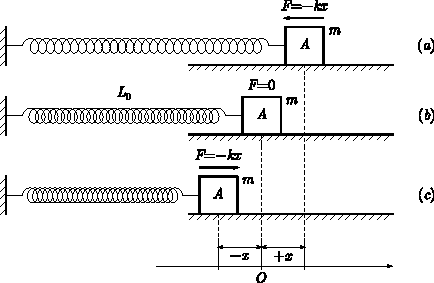
\includegraphics{figure/fig03.03}
    \caption{弹性力}
    \label{fig:03.03}
\end{figurex}
% 097.jpg

一个倔强系数为$ k $的弹簧和物体$ A $相连,弹簧固有长度为$ L _ { 0 } $
〔图\ref{fig:03.03}(b)〕。在这个位置,弹簧对$ A $不施力,称为平衡位置,取
其为坐标原点。如果$ A $向右移动〔图\ref{fig:03.03}(a)〕,则弹簧将对物体$ A $施
向左之力,此力的大小为
\begin{equation}\label{eqn:03.04.01}
    F = - k x
\end{equation}
如果将$ A $向左移动〔图\ref{fig:03.03}(c)〕,则弹簧对$ A $施之力就指向右
边,而此力为
\begin{equation*}
    F = - k x
\end{equation*}
在这两种情况下,它对$ A $所施之力都指向平衡位置,故称其为回
复力。

\heiti 2. 摩擦力 \normalfont

\begin{wrapfigure}[8]{r}{13em}
    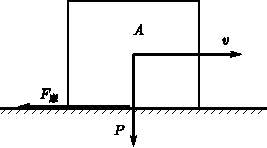
\includegraphics{figure/fig03.04}
    \caption{摩擦力}
    \label{fig:03.04}
\end{wrapfigure}
摩擦力是最常遇到的一种力,但是关于它的规律却是异常
复杂的。我们在这里仅谈几条简单的规律。如图\ref{fig:03.04}~所示,两个固
态物体之间的摩擦力$ \vec{F}_\text{摩} $,方向与运动或运动趋势的方向相反,
在一定范围内,大小正比于两物体之间的正压力$ P $,即\vspace{-0.2em}
\begin{equation}\label{eqn:03.04.02}
    F_\text{摩} = \mu P
\end{equation}

\begin{wrapfigure}[7]{l}{13em}
    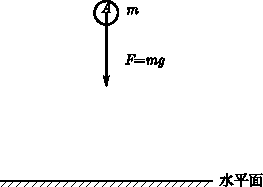
\includegraphics{figure/fig03.05}
    \caption{重力}
    \label{fig:03.05}
\end{wrapfigure}
\noindent 其中$\mu$称为摩擦系数。一般说来,滚动摩擦系数小于滑动摩擦系
数;运动状态的摩擦系数小于静止状态的摩擦系数。

\heiti 3. 重力 \normalfont

我们对重力也很熟悉,如图\ref{fig:03.05}~所示,在地球表面附近,一个
质量为$ m $的物体受到的重力方向
% 098.jpg
垂直于水平面,大小为
\begin{equation}\label{eqn:03.04.03}
    F = m g
\end{equation}
其中$ g $是重力加速度。

\heiti 4. 万有引力 \normalfont

第四章将专题讨论。

\heiti 5. 库仑力 \normalfont

带电体之间的相互作用规律是由法国物理学家库仑发现的,
\begin{wrapfigure}[4]{r}{13em}
    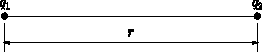
\includegraphics{figure/fig03.06}
    \caption{库仑力}
    \label{fig:03.06}
\end{wrapfigure}
因而称之为库仑力。一个静止的点电荷要吸引或排斥另一静止的
点电荷,力的大小与电荷的乘积成正比,与它们之间的距离的平
方成反比,方向沿着两点电荷的连线。如果电荷是异号的,则为
吸引力;如果是同号的,则是排斥力。如图\ref{fig:03.06}~所示,库仑力的大
小为
\begin{equation}\label{eqn:03.04.04}
    F = \kappa \frac { q _ { 1 } q _ { 2 } } { r ^ { 2 } }
\end{equation}
其中$ \kappa $是比例系数,$  q _ { 1 } $,$  q _ { 2 } $是两质点的电荷

\heiti 6. 分子力 \normalfont

分子间相互作用的规律较复杂,很难用简单的数学公式来表
示。一般在实验的基础上,采用简化模型处理问题,可近似地用
下列的半经验公式来表示:
\begin{equation}\label{eqn:03.04.05}
    F = \frac { \lambda } { r ^ { s } } - \frac { \mu } { r ^ t } \quad \left( s > t \right)
\end{equation}
式中为两个分子中心之间的距离;$\lambda$,$\mu$,$ s $,$ t $都是正数(需根据
实验数据加以确定)。式\eqref{eqn:03.04.05}中的第一项是正的,代表斥力
第二项是负的,代表引力。由于$ s $和$ t $都比较大,$ t $一般约为$ 6\sim 7 $,
所以分子力随分子间距离$ r $的增大而急剧地减小。这种力可以认
为具有一定的有效作用距离,超出有效作用距离,作用力实际上
% 099.jpg
\begin{wrapfigure}[11]{r}{13em}
    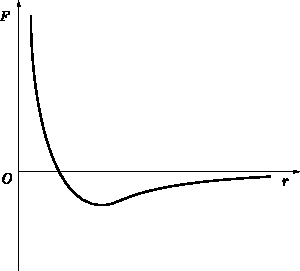
\includegraphics{figure/fig03.07}
    \caption{分子力}
    \label{fig:03.07}
\end{wrapfigure}
可以完全忽略。由于$  s > t   $,所以斥力的有效作用距离比引力的小力随的变化情况大致如图\ref{fig:03.07}~所示。

\heiti 7. 核力 \normalfont

核力是把原子核中的核子(质子和中子)束缚在一起的力。
这种力有效作用距离极短,对于大于约\num{1e-13}厘米的距离,核力很
快就变得很小,可略而不计了。但在小尺度内,它却超过核子之
间的一切其他形式的相互作占支配地位。这是一种异常复杂
类型的相互作用,直到大约\num{0.4e-13}厘米,它还是吸引力,大小可表示为
\begin{equation}\label{eqn:03.04.06}
    F = \frac { C } { r ^ { n } } \e ^ { - \frac { r } { r_0 } }
\end{equation}
其中$ C $,$ n $为常数;$ r $是两个核子间的距离, $ r _ { 0 } \approx \num{e-13} $厘米。但距
离若是再小,就成为强排斥力了。

\heiti 8. 洛伦兹力 \normalfont

一个带电荷\,$ q $\,的点电荷以速度\,$\vec{v}$\,在磁感应强度为\,$\vec{B}$\,的磁场中
运动,要受到磁场的作用力,此种力称为洛伦兹力,其表达式为:
\begin{equation}\label{eqn:03.04.07}
    \vec{F} = q \vec{v} \times \vec{B}
\end{equation}

\heiti 9. 粘滞力 \normalfont

物体在流体(液体或气体)中运动时,受到阻力。这种力是流
体粘滞性的一种表示。当运动物体速度不太大时,粘滞力可表示
为:\vspace{-1em}
\begin{equation}\label{eqn:03.04.08}
    \vec{F} = - \eta \vec{v}
\end{equation}
其中系数$\eta$表示粘滞性,负号表示粘滞力与运动方向相反。
% 100.jpg

以上我们列举了九种力,当然,还可以举出很多种。在绪论
中,我们指出,物理学并不仅仅满足于把各式各样的力罗列出
来,因为,物理学认为客观世界的现象虽是复杂的,但原因却是
简单的。从本质上讲,自然界并不存在如此多种类型的力,我们
希望寻求各种现象的统一。在目前的宇宙中,存在着四类基本的
相互作用,所有的运动现象的原因都逃不出这四类基本的力,各
式各样的力只不过是这四类基本力在不同情况下的不同表现而
已。四类基本作用是:引力作用、电磁作用、强相互作用、弱相
互作用。而在宇宙的早期,这些力之间表现的不同可能也不存在,
它们逐步合成最基本的力。例如,在宇宙年龄约1秒之前,电磁
作用和弱相互作用的差别可能完全消失了。



